\section{Requisitos}
En la tabla \ref{table:requisitos} se muestran los requisitos del sistema desarrollado.

\begin{table}[H]
\centering
\begin{tabular}{|c|l|l|}
\hline
\rowcolor[HTML]{EFEFEF} 
\textbf{Grupo}                                                                                  & \multicolumn{1}{c|}{\cellcolor[HTML]{EFEFEF}\textbf{ID}} & \multicolumn{1}{c|}{\cellcolor[HTML]{EFEFEF}\textbf{Descripción}}                 \\ \hline
                                                                                                & 1.1                                                      & Implementación de receta de carbonatación según ISA S88.                          \\ \cline{2-3} 
                                                                                                & 1.2                                                      & Inyección de CO2 mediante válvula solenoide (QMB1).                               \\ \cline{2-3} 
                                                                                                & 1.3                                                      & Disolución de CO2 mediante criba vibratoria accionada por motor eléctrico (MAA1). \\ \cline{2-3} 
\multirow{-4}{*}{Control del proceso}                                                           & 1.4                                                      & Monitoreo de presión (BPA1).                                                      \\ \hline
                                                                                                & 2.1                                                      & Comunicación con MCU.                                                             \\ \cline{2-3} 
                                                                                                & 2.2                                                      & Indicación de estado de receta.                                                   \\ \cline{2-3} 
                                                                                                & 2.3                                                      & Indicación de paso de receta.                                                     \\ \cline{2-3} 
                                                                                                & 2.4                                                      & Indicación de alarmas.                                                            \\ \cline{2-3} 
                                                                                                & 2.5                                                      & Indicación de presión BPA1.                                                       \\ \cline{2-3} 
\multirow{-6}{*}{HMI}                                                                           & 2.6                                                      & Botones de comando de receta: start, stop, hold, resume, reset.                   \\ \hline
                                                                                                & 3.1                                                      & Conexión con MCU.                                                                 \\ \cline{2-3} 
\multirow{-2}{*}{Sirena}                                                                        & 3.2                                                      & Configuración de la alerta sonora.                                                \\ \hline
                                                                                                & 4.1                                                      & Comunicación con MCU.                                                             \\ \cline{2-3} 
                                                                                                & 4.2                                                      & Comandos de receta: start, stop, hold, resume, reset.                             \\ \cline{2-3} 
                                                                                                & 4.3                                                      & Comando de reporte de presión BPA1.                                               \\ \cline{2-3} 
\multirow{-4}{*}{\begin{tabular}[c]{@{}c@{}}Computadora de\\ supervisión\end{tabular}}          & 4.4                                                      & Comando de ayuda al operador.                                                     \\ \hline
                                                                                                & 5.1                                                      & Alarma por sobrepresión cuando \(BPA1 > 4\,bar\).                                 \\ \cline{2-3} 
\multirow{-2}{*}{\begin{tabular}[c]{@{}c@{}}Sistema de alarmas\\ y enclavamientos\end{tabular}} & 5.2                                                      & Detención del proceso por sobrepresión cuando \(BPA1 > 4\,bar\).                  \\ \hline
                                                                                                & 6.1                                                      & Comunicación WiFi con MCU.                                                        \\ \cline{2-3} 
                                                                                                & 6.2                                                      & Implementación de servidor HTTP.                                                  \\ \cline{2-3} 
                                                                                                & 6.3                                                      & Indicación de estado de receta mediante HTML.                                     \\ \cline{2-3} 
                                                                                                & 6.4                                                      & Indicación de paso de receta.                                                     \\ \cline{2-3} 
                                                                                                & 6.5                                                      & Indicación de presión BPA1.                                                       \\ \cline{2-3} 
\multirow{-6}{*}{Servidor web}                                                                  & 6.6                                                      & Indicación de alarmas.                                                            \\ \hline
\end{tabular}
\caption{Requisitos del sistema automático.}
\label{table:requisitos}
\end{table}


\section{Casos de uso}
En las tablas \ref{table:caso-de-uso-1}, \ref{table:caso-de-uso-2} y \ref{table:caso-de-uso-3} se presentan tres casos de uso del sistema representativos de su funcionalidad.

\begin{table}[H]
\centering
\begin{tabular}{|
>{\columncolor[HTML]{EFEFEF}}l |l|}
\hline
\textbf{Caso de uso}       & Inicio de receta de carbonatación                                                                                                                                                        \\ \hline
\textbf{Descripción}       & El operador inicia la receta para carbonatar un barril de cerveza.                                                                                                                       \\ \hline
\textbf{Precondición}      & La receta debe estar en el estado Idle y el sistema no debe estar enclavado.                                                                                                             \\ \hline
\textbf{Flujo principal}   & \begin{tabular}[c]{@{}l@{}}1. El operador selecciona Start en el HMI.\\ 2. El sistema inicia la receta.\\ 3. Se inyecta \(CO_{2}\) y se agita el barril según el algoritmo.\end{tabular} \\ \hline
\textbf{Flujo alternativo} & \begin{tabular}[c]{@{}l@{}}Si se detecta \(BPA1 > 4\,bar\), se activa la alarma, se detiene el proceso y se\\ notifica al operador.\end{tabular}                                         \\ \hline
\end{tabular}
\caption{Caso de uso 1, inicio de la ejecución de la receta.}
\label{table:caso-de-uso-1}
\end{table}

\begin{table}[H]
\centering
\begin{tabular}{|
>{\columncolor[HTML]{EFEFEF}}l |l|}
\hline
\textbf{Caso de uso}       & Pausa y reanudación de receta                                                                                                                                                                    \\ \hline
\textbf{Descripción}       & El operador pausa temporalmente la receta en ejecución y luego la reanuda.                                                                                                                       \\ \hline
\textbf{Precondición}      & La receta debe estar en el estado Executing.                                                                                                                                                     \\ \hline
\textbf{Flujo principal}   & \begin{tabular}[c]{@{}l@{}}1. El operador selecciona Hold en el HMI.\\ 2. El sistema detiene la operación de los actuadores.\\ 3. Posteriormente, selecciona Resume para continuar.\end{tabular} \\ \hline
\textbf{Flujo alternativo} & \begin{tabular}[c]{@{}l@{}}Si la presión en el barril cambia mientras está pausado, \\ se realiza una notificación visual en el HMI.\end{tabular}                                                \\ \hline
\end{tabular}
\caption{Caso de uso 2, pausa y reanudación de receta}
\label{table:caso-de-uso-2}
\end{table}

\begin{table}[H]
\centering
\begin{tabular}{|
>{\columncolor[HTML]{EFEFEF}}l |l|}
\hline
\textbf{Caso de uso}       & Reporte de presión BPA1 a la computadora de supervisión.                                                                                                                                                                                             \\ \hline
\textbf{Descripción}       & \begin{tabular}[c]{@{}l@{}}El operador se conecta a la computadora de supervisión comandando el\\ reporte de la presión BPA1.\end{tabular}                                                                                                           \\ \hline
\textbf{Precondición}      & La computadora de supervisión debe estar conectada a la interfaz UART.                                                                                                                                                                               \\ \hline
\textbf{Flujo principal}   & \begin{tabular}[c]{@{}l@{}}1. El operador envía el comando 'r' para inicial el reporte de la presión.\\ 2. Se envía la presión BPA1 en un payload de JSON.\\ 3. El operador envía el comando 'R' para detener el reporte de la presión.\end{tabular} \\ \hline
\textbf{Flujo alternativo} & \multicolumn{1}{c|}{-}                                                                                                                                                                                                                               \\ \hline
\end{tabular}
\caption{Caso de uso 3, reporte de presión BPA1 a la computadora de supervisión a través del terminal serie.}
\label{table:caso-de-uso-3}
\end{table}

\section{Descripción de módulos utilizados}
En base a la arquitectura de control y los requisitos establecidos se decidió por utilizar los módulos que se describen a continuación.

\subsection{Módulo del microcontrolador}
Se utilizó como módulo microcontrolador la placa NUCLEO-F429ZI \cite{NUCLEO}, equipada con un microcontrolador STM32F429ZI, figura \ref{fig:nucleo}.

Los principales puntos tenidos en cuenta para la adopción de esta placa son:
\begin{itemize}
\item Rendimiento y recursos: El STM32F429ZI incluye un núcleo ARM Cortex-M4 de alto rendimiento con capacidad de punto flotante, ideal para realizar cálculos en tiempo real y ejecutar múltiples tareas simultáneamente.
\item Periféricos integrados: La placa cuenta con una amplia gama de periféricos como UART, SPI, ADC y GPIO, que permiten una integración eficiente con los sensores y actuadores del sistema.
\item Compatibilidad con herramientas de desarrollo: La placa es compatible con Mbed OS y herramientas como STM32CubeIDE, lo que facilita el desarrollo del software.
\item Documentación y soporte: La disponibilidad de documentación detallada simplifica el proceso de implementación y resolución de problemas.
\end{itemize}

\begin{figure}[H]
  \centering
  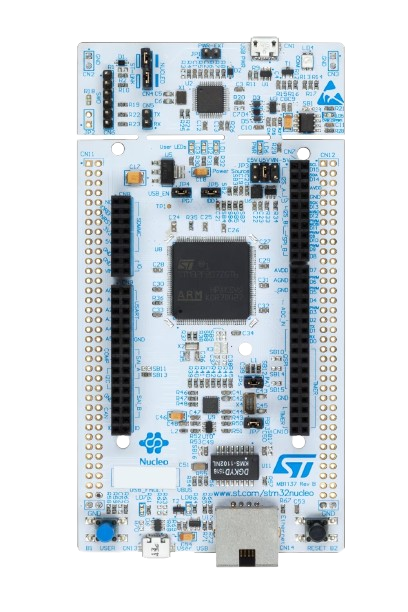
\includegraphics[width=0.5\linewidth]{introduccion-especifica/img/nucleo.png}
  \caption{NUCLEO-F429ZI.}
  \label{fig:nucleo}
\end{figure}

\subsection{Módulo del display táctil}
Para la implementación del HMI se utilizó el módulo display \cite{LCD} con pantalla LCD TFT de 2.4' y drivers de hardware ILI9341 y XPT2046 que se muestra en la figura \ref{fig:hmi}.

El comando gráfico del LCD se realiza con el hardware ILI9341 a través de una comunicación SPI y el comando de la interacción táctil con el hardware XPT2046 también a través de una comunicación SPI.

\begin{figure}[H]
  \centering
  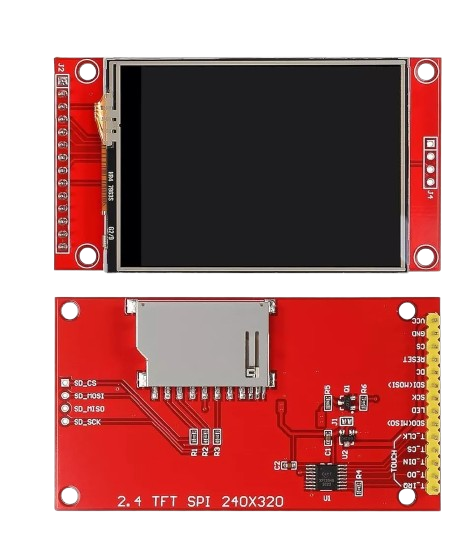
\includegraphics[width=0.5\linewidth]{introduccion-especifica/img/hmi.png}
  \caption{Modulo display táctil.}
  \label{fig:hmi}
\end{figure}

\subsection{Módulo Wi-Fi}
Para la implementación de la comunicación con la computadora de supervisión a través de un navegador web se utiliza el módulo Wi-Fi ESP01 \cite{ESP01} de la figura \ref{fig:esp01}.

Este módulo se comunica con el microcontrolador a través de una interfaz UART y la configuración del mismo se realiza a través de comandos AT.

\begin{figure}[H]
  \centering
  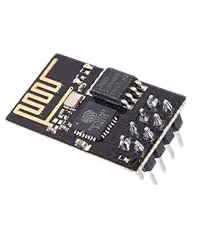
\includegraphics[width=0.35\linewidth]{introduccion-especifica/img/ESP01.png}
  \caption{Modulo ESP01.}
  \label{fig:esp01}
\end{figure}

\subsection{Buzzer}
Para las indicaciones auditivas se utiliza el buzzer pasivo KY-006 que se muestra en la figura \ref{fig:buzzer}. El dispositivo se activa enviando una señal PWM al terminal de entrada.

\begin{figure}[H]
  \centering
  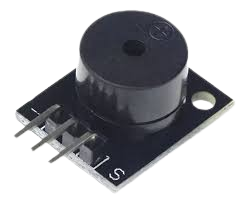
\includegraphics[width=0.35\linewidth]{introduccion-especifica/img/buzzer.png}
  \caption{Buzzer}
  \label{fig:buzzer}
\end{figure}

\subsection{Módulo de alimentación}
Para la alimentación de los módulos de display, Wi-Fi y el buzzer se utiliza el módulo MB102 que se muestra en la figura \ref{fig:mb102}. El dispositivo genera \(3.3\,V\) al conectar el USB de entrada a \(5\,V\).

\begin{figure}[H]
  \centering
  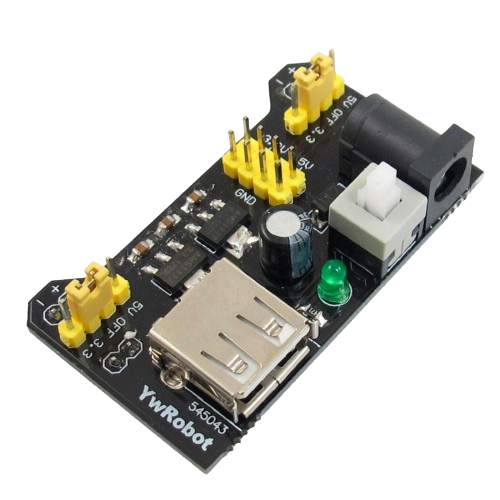
\includegraphics[width=0.35\linewidth]{introduccion-especifica/img/mb102.png}
  \caption{Módulo de alimentación MB102.}
  \label{fig:mb102}
\end{figure}

%%% Local Variables:
%%% mode: latex
%%% TeX-master: "../main"
%%% End:
